\documentclass{standalone}
\usepackage{tikz}
\usetikzlibrary{patterns, positioning}

\begin{document}
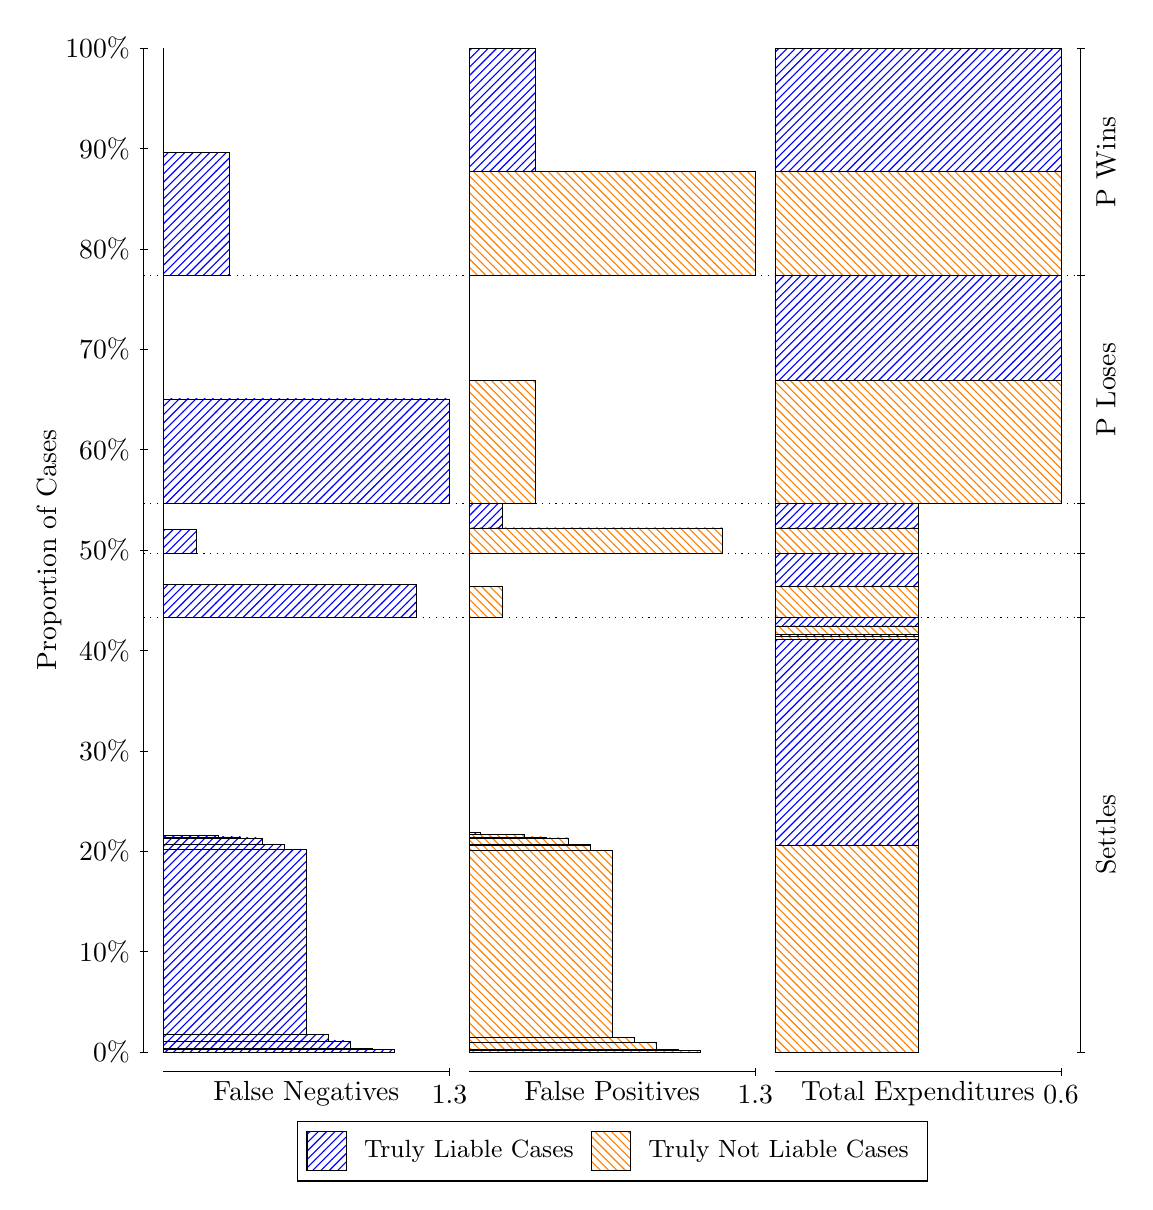
\begin{tikzpicture}
\draw[black, very thin] (1.5,1.75) -- (1.5,14.5);
\node[rotate=90, anchor=center] at (0.3, 8.125) {Proportion of Cases};
\draw[black, very thin] (1.45,1.75) -- (1.55,1.75);
\node[anchor=east] at (1.45, 1.75) {0\%};
\draw[black, very thin] (1.45,3.025) -- (1.55,3.025);
\node[anchor=east] at (1.45, 3.025) {10\%};
\draw[black, very thin] (1.45,4.3) -- (1.55,4.3);
\node[anchor=east] at (1.45, 4.3) {20\%};
\draw[black, very thin] (1.45,5.575) -- (1.55,5.575);
\node[anchor=east] at (1.45, 5.575) {30\%};
\draw[black, very thin] (1.45,6.85) -- (1.55,6.85);
\node[anchor=east] at (1.45, 6.85) {40\%};
\draw[black, very thin] (1.45,8.125) -- (1.55,8.125);
\node[anchor=east] at (1.45, 8.125) {50\%};
\draw[black, very thin] (1.45,9.4) -- (1.55,9.4);
\node[anchor=east] at (1.45, 9.4) {60\%};
\draw[black, very thin] (1.45,10.675) -- (1.55,10.675);
\node[anchor=east] at (1.45, 10.675) {70\%};
\draw[black, very thin] (1.45,11.95) -- (1.55,11.95);
\node[anchor=east] at (1.45, 11.95) {80\%};
\draw[black, very thin] (1.45,13.225) -- (1.55,13.225);
\node[anchor=east] at (1.45, 13.225) {90\%};
\draw[black, very thin] (1.45,14.5) -- (1.55,14.5);
\node[anchor=east] at (1.45, 14.5) {100\%};

\draw[black, very thin] (13.4,1.75) -- (13.4,14.5);
\draw[black, very thin] (13.35,1.75) -- (13.45,1.75);
\node[anchor=west] at (13.35, 1.75) {};
\draw[black, very thin] (13.35,7.2691) -- (13.45,7.2691);
\node[anchor=west] at (13.35, 7.2691) {};
\draw[black, very thin] (13.35,8.0804) -- (13.45,8.0804);
\node[anchor=west] at (13.35, 8.0804) {};
\draw[black, very thin] (13.35,8.7153) -- (13.45,8.7153);
\node[anchor=west] at (13.35, 8.7153) {};
\draw[black, very thin] (13.35,11.608) -- (13.45,11.608);
\node[anchor=west] at (13.35, 11.608) {};
\draw[black, very thin] (13.35,14.5) -- (13.45,14.5);
\node[anchor=west] at (13.35, 14.5) {};

\draw[black, very thin, pattern color=blue, pattern=north east lines] (1.75,1.75) rectangle (4.6846,1.7835);
\draw[black, very thin, pattern color=blue, pattern=north east lines] (1.75,1.7835) rectangle (4.4051,1.7974);
\draw[black, very thin, pattern color=blue, pattern=north east lines] (1.75,1.7974) rectangle (4.1256,1.8899);
\draw[black, very thin, pattern color=blue, pattern=north east lines] (1.75,1.8899) rectangle (3.8462,1.9704);
\draw[black, very thin, pattern color=blue, pattern=north east lines] (1.75,1.9704) rectangle (3.5667,4.3231);
\draw[black, very thin, pattern color=blue, pattern=north east lines] (1.75,4.3231) rectangle (3.2872,4.3901);
\draw[black, very thin, pattern color=blue, pattern=north east lines] (1.75,4.3901) rectangle (3.0077,4.4683);
\draw[black, very thin, pattern color=blue, pattern=north east lines] (1.75,4.4683) rectangle (2.7282,4.482);
\draw[black, very thin, pattern color=blue, pattern=north east lines] (1.75,4.482) rectangle (2.4487,4.505);
\draw[black, very thin, pattern color=orange, pattern=north west lines] (1.75,4.505) rectangle (1.75,7.2691);
\draw[black, very thin, pattern color=blue, pattern=north east lines] (1.75,7.2691) rectangle (4.9641,7.6873);
\draw[black, very thin, pattern color=orange, pattern=north west lines] (1.75,7.6873) rectangle (1.75,8.0804);
\draw[black, very thin, pattern color=blue, pattern=north east lines] (1.75,8.0804) rectangle (2.1692,8.3908);
\draw[black, very thin, pattern color=orange, pattern=north west lines] (1.75,8.3908) rectangle (1.75,8.7153);
\draw[black, very thin, pattern color=blue, pattern=north east lines] (1.75,8.7153) rectangle (5.3833,10.043);
\draw[black, very thin, pattern color=orange, pattern=north west lines] (1.75,10.043) rectangle (1.75,11.608);
\draw[black, very thin, pattern color=blue, pattern=north east lines] (1.75,11.608) rectangle (2.5885,13.171);
\draw[black, very thin, pattern color=orange, pattern=north west lines] (1.75,13.171) rectangle (1.75,14.5);
\draw[black, very thin, pattern color=orange, pattern=north west lines] (5.6333,1.75) rectangle (8.5679,1.773);
\draw[black, very thin, pattern color=orange, pattern=north west lines] (5.6333,1.773) rectangle (8.2885,1.787);
\draw[black, very thin, pattern color=orange, pattern=north west lines] (5.6333,1.787) rectangle (8.009,1.8686);
\draw[black, very thin, pattern color=orange, pattern=north west lines] (5.6333,1.8686) rectangle (7.7295,1.9386);
\draw[black, very thin, pattern color=orange, pattern=north west lines] (5.6333,1.9386) rectangle (7.45,4.3062);
\draw[black, very thin, pattern color=orange, pattern=north west lines] (5.6333,4.3062) rectangle (7.1705,4.3796);
\draw[black, very thin, pattern color=orange, pattern=north west lines] (5.6333,4.3796) rectangle (7.1705,4.3817);
\draw[black, very thin, pattern color=orange, pattern=north west lines] (5.6333,4.3817) rectangle (6.891,4.4687);
\draw[black, very thin, pattern color=orange, pattern=north west lines] (5.6333,4.4687) rectangle (6.6115,4.482);
\draw[black, very thin, pattern color=orange, pattern=north west lines] (5.6333,4.482) rectangle (6.3321,4.5141);
\draw[black, very thin, pattern color=blue, pattern=north east lines] (5.6333,4.5141) rectangle (5.7731,4.5371);
\draw[black, very thin, pattern color=blue, pattern=north east lines] (5.6333,4.5371) rectangle (5.6333,7.2691);
\draw[black, very thin, pattern color=orange, pattern=north west lines] (5.6333,7.2691) rectangle (6.0526,7.6622);
\draw[black, very thin, pattern color=blue, pattern=north east lines] (5.6333,7.6622) rectangle (5.6333,8.0804);
\draw[black, very thin, pattern color=orange, pattern=north west lines] (5.6333,8.0804) rectangle (8.8474,8.4049);
\draw[black, very thin, pattern color=blue, pattern=north east lines] (5.6333,8.4049) rectangle (6.0526,8.7153);
\draw[black, very thin, pattern color=orange, pattern=north west lines] (5.6333,8.7153) rectangle (6.4718,10.28);
\draw[black, very thin, pattern color=blue, pattern=north east lines] (5.6333,10.28) rectangle (5.6333,11.608);
\draw[black, very thin, pattern color=orange, pattern=north west lines] (5.6333,11.608) rectangle (9.2667,12.937);
\draw[black, very thin, pattern color=blue, pattern=north east lines] (5.6333,12.937) rectangle (6.4718,14.5);
\draw[black, very thin, pattern color=orange, pattern=north west lines] (9.5167,1.75) rectangle (11.333,4.3796);
\draw[black, very thin, pattern color=blue, pattern=north east lines] (9.5167,4.3796) rectangle (11.333,6.9925);
\draw[black, very thin, pattern color=orange, pattern=north west lines] (9.5167,6.9925) rectangle (11.333,7.0246);
\draw[black, very thin, pattern color=blue, pattern=north east lines] (9.5167,7.0246) rectangle (11.333,7.0581);
\draw[black, very thin, pattern color=orange, pattern=north west lines] (9.5167,7.0581) rectangle (11.333,7.1605);
\draw[black, very thin, pattern color=blue, pattern=north east lines] (9.5167,7.1605) rectangle (11.333,7.2691);
\draw[black, very thin, pattern color=orange, pattern=north west lines] (9.5167,7.2691) rectangle (11.333,7.6622);
\draw[black, very thin, pattern color=blue, pattern=north east lines] (9.5167,7.6622) rectangle (11.333,8.0804);
\draw[black, very thin, pattern color=orange, pattern=north west lines] (9.5167,8.0804) rectangle (11.333,8.4049);
\draw[black, very thin, pattern color=blue, pattern=north east lines] (9.5167,8.4049) rectangle (11.333,8.7153);
\draw[black, very thin, pattern color=orange, pattern=north west lines] (9.5167,8.7153) rectangle (13.15,10.28);
\draw[black, very thin, pattern color=blue, pattern=north east lines] (9.5167,10.28) rectangle (13.15,11.608);
\draw[black, very thin, pattern color=orange, pattern=north west lines] (9.5167,11.608) rectangle (13.15,12.937);
\draw[black, very thin, pattern color=blue, pattern=north east lines] (9.5167,12.937) rectangle (13.15,14.5);
\draw[black, dotted] (1.5,7.2691) -- (13.4,7.2691);
\draw[black, dotted] (1.5,8.0804) -- (13.4,8.0804);
\draw[black, dotted] (1.5,8.7153) -- (13.4,8.7153);
\draw[black, dotted] (1.5,11.608) -- (13.4,11.608);
\draw[black, very thin] (1.75,1.5) -- (5.3833,1.5);
\node[anchor=north] at (3.5667, 1.5) {False Negatives};
\draw[black, very thin] (5.3833,1.45) -- (5.3833,1.55);
\node[anchor=north] at (5.3833, 1.45) {1.3};

\draw[black, very thin] (5.6333,1.5) -- (9.2667,1.5);
\node[anchor=north] at (7.45, 1.5) {False Positives};
\draw[black, very thin] (9.2667,1.45) -- (9.2667,1.55);
\node[anchor=north] at (9.2667, 1.45) {1.3};

\draw[black, very thin] (9.5167,1.5) -- (13.15,1.5);
\node[anchor=north] at (11.333, 1.5) {Total Expenditures};
\draw[black, very thin] (13.15,1.45) -- (13.15,1.55);
\node[anchor=north] at (13.15, 1.45) {0.6};

\node[black, centered, rotate=90] at (13.72, 4.5096) {Settles};


\node[black, centered, rotate=90] at (13.72, 10.162) {P Loses};
\node[black, centered, rotate=90] at (13.72, 13.054) {P Wins};

\draw (7.449999999999999,1.5) node[draw=none] (baseCoordinate) {};
\begin{scope}[align=center]
        \matrix[scale=0.5, draw=black, below=0.5cm of baseCoordinate, nodes={draw}, column sep=0.1cm]{
            \node[rectangle, draw, minimum width=0.5cm, minimum height=0.5cm, pattern=north east lines, pattern color=blue] {}; &
            \node[draw=none, font=\small] (B) {Truly Liable Cases}; &
            \node[rectangle, draw, minimum width=0.5cm, minimum height=0.5cm, pattern=north west lines, pattern color=orange] {}; &
            \node[draw=none, font=\small] (B) {Truly Not Liable Cases}; \\
            };
\end{scope}

\end{tikzpicture}
\end{document}